\documentclass[uplatex,dvipdfmx]{jsarticle}
\usepackage{listings,jvlisting}
\usepackage{color}
\usepackage{xr}

\lstset{
  backgroundcolor=\color[rgb]{0.9,0.9,0.9},
  frame=single,
  basicstyle=\ttfamily
}
\makeatletter

\newcommand{\pr}[1]{\colorbox[rgb]{0.9,0.9,0.9}{\lstinline{#1}}}
\newcommand{\functype}[2]{\pr{#1 -> #2}}
\newcommand{\refcti}[1]{[CTI]\ref{#1}}
\newcommand{\fpmor}[3]{\pr{#1 :: #2 -> #3}}
\input{../categoryTheoryIntro/preemble.tex}
\begin{document}
  \title{Profunctorの表現定理の仮まとめ}

  $\cat{Prof} := \funccat{C^{op}\times C}{Set}$とする。

  \begin{prop}[Profunctorの表現定理]
    \[\coend{C}{M}\arset{C}{S}{M\otimes A}\times\arset{C}{M\otimes A'}{S'}\cong\cend{Tamb}{T}\arset{Set}{U(T)(A,A')}{U(T)(S,S')}\]
  \end{prop}

  この命題の$\cat{Tamb}$は追加の構造を持ったProfunctorのなす圏のことであり、$U(T)$は$T$から追加の構造を忘れた単なるProfunctorである。圏$\cat{Tamb}$を定義する前にこの追加の構造について説明する。

  \section{丹原加群と余EM圏}
  まずモノイダル積関手$\mor{M\otimes -}{C}{C}$における射関数は\[\mor{M\otimes -}{\arset{C}{A}{A'}}{\arset{C}{M\otimes A}{M\otimes A'}}\]というような射であるが、これを双Hom関手$\functor{\arset{C}{-}{-}}{C^{op}\times C}{Set}$からProfunctorへ拡張して
  \[\mor{\zeta_{A,A',M}}{P(A,A')}{P(M\otimes A, M\otimes A')}\]となるような射を考える。またモノイダル積関手の射関数では、射関数の自然性から$A,A'$に対して自然であったから$\zeta$にも$A,A'$に対する自然性を課す。さらに射$\mor{f}{M}{N}$に対してモノイダル積関手の間の自然変換$\nat{f\otimes -}{M\otimes -}{N\otimes -}$を考えることができたから、その成分に該当する$\zeta$にも$M$に対する自然性を課したい。しかし$P(M\otimes A,M\otimes A')$や$P(N\otimes A, N\otimes A')$は射集合ではないから代わりに超自然性と呼ばれる一般化された自然性を課す。

  \begin{define}
    関手$\functor{F}{C^{op}\times C}{Set}$に対して対象$X$、$\mor{\mu_A}{X}{F(A,A)}$が楔$(X,\mu)$である時、$\mu$を超自然変換と呼ぶ。
    また対象$X$、$\mor{\mu_A}{F(A,A)}{X}$が余楔$(X,\mu)$である時も同様に超自然変換と呼ぶ。
  \end{define}
  \begin{center}
    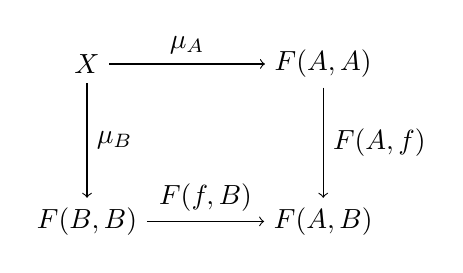
\begin{tikzpicture}[auto]
      \node (FG) at (0, 0) {$X$};
      \node (FAGA) at (3, 0) {$F(A,A)$};
      \node (FBGB) at (0, -2) {$F(B,B)$};
      \node (FAGB) at (3, -2) {$F(A,B)$};

      \draw[->] (FG) to node{$\mu_A$}(FAGA);
      \draw[->] (FG) to node{$\mu_B$}(FBGB);
      \draw[->] (FAGA) to node{$F(A,f)$}(FAGB);
      \draw[->] (FBGB) to node{$F(f,B)$}(FAGB);
    \end{tikzpicture}
  \end{center}
  自然変換がエンドで定義されることから、自然変換の成分を元と見なした時これらは超自然性を持つ。
  \begin{center}
    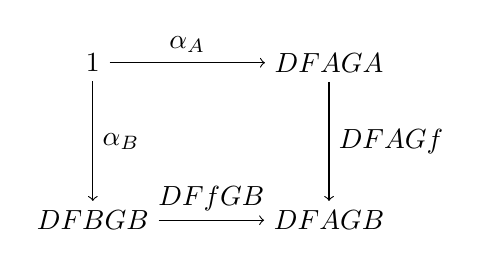
\begin{tikzpicture}[auto]
      \node (FG) at (0, 0) {$1$};
      \node (FAGA) at (3, 0) {$\arset{D}{FA}{GA}$};
      \node (FBGB) at (0, -2) {$\arset{D}{FB}{GB}$};
      \node (FAGB) at (3, -2) {$\arset{D}{FA}{GB}$};

      \draw[->] (FG) to node{$\alpha_A$}(FAGA);
      \draw[->] (FG) to node{$\alpha_B$}(FBGB);
      \draw[->] (FAGA) to node{$\arset{D}{FA}{Gf}$}(FAGB);
      \draw[->] (FBGB) to node{$\arset{D}{Ff}{GB}$}(FAGB);
    \end{tikzpicture}
  \end{center}
  またエンドの定義よりエンド$(\cend{C}{C} F(C,C),\tau)$が存在する時、任意の楔$(X,\mu)$に対して射$\mor{h}{X}{\cend{C}{C} F(C,C)}$が一意に存在する。すなわち、$A$に対して超自然な射$\mor{\mu_A}{X}{F(A,A)}$の全体は\[\arset{C}{X}{\cend{C}{C} F(C,C)}\]と表すことができる。

  $\zeta$の話に戻ると、$N$に対する超自然性は以下の図式で表され、
  \begin{center}
    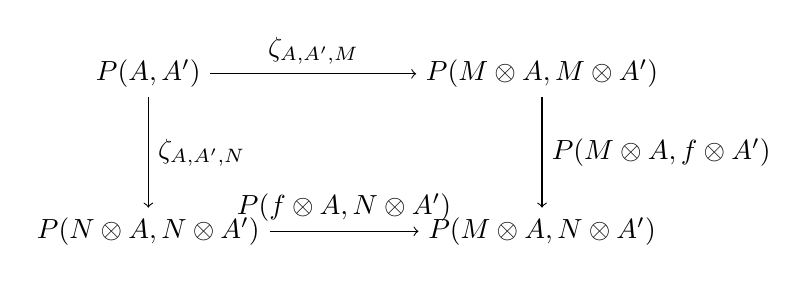
\begin{tikzpicture}[auto]
      \node (FG) at (0, 0) {$P(A,A')$};
      \node (FAGA) at (5, 0) {$P(M\otimes A,M\otimes A')$};
      \node (FBGB) at (0, -2) {$P(N\otimes A,N\otimes A')$};
      \node (FAGB) at (5, -2) {$P(M\otimes A,N\otimes A')$};

      \draw[->] (FG) to node{$\zeta_{A,A',M}$}(FAGA);
      \draw[->] (FG) to node{$\zeta_{A,A',N}$}(FBGB);
      \draw[->] (FAGA) to node{$P(M\otimes A, f\otimes A')$}(FAGB);
      \draw[->] (FBGB) to node{$P(f\otimes A, N\otimes A')$}(FAGB);
    \end{tikzpicture}
  \end{center}
  さらに$M$を束縛すると、$\mor{\zeta_{A,A'}}{P(A,A')}{\cend{C}{M}P(M\otimes A, M\otimes A')}$となるような射が得られる。  

  \begin{prop}
    Profunctor $\profunctor{P}{C}{C}$に対して\[\Theta(P) = \cend{C}{M}P(M\otimes -, M\otimes -)\]とすると、$\Theta(P)$はProfunctor $\profunctor{\Theta P}{C}{C}$であり、$\Theta$は関手$\functor{\Theta}{Prof}{Prof}$である。
  \end{prop}
  \begin{proof}
    $P$はProfunctorであり、$M\otimes -$の関手性とコエンドの普遍性から$\Theta(P)$もProfuctorになる。$\Theta$の関手性もコエンドの普遍性より成り立つ。
  \end{proof}
  \begin{define}[コモナド]
    関手$\functor{W}{C}{C}$に対するコモナド$(T,\delta, \epsilon)$を以下の要素で構成する。
    \begin{quote}
      \begin{mydescription}
        \item[余乗算子] 自然変換$\nat{\delta}{W}{W\circ W}$
        \item[余単位子] 自然変換$\nat{\epsilon}{W}{Id_W}$
        \item[余結合則] 以下の図式を可換にする。
        \begin{center}
          \begin{tikzpicture}[auto]
            \node (w) at (0, 0) {$W$};
            \node (ww) at (3, 0) {$W\circ W$};
            \node (ww2) at (0, -2) {$W\circ W$};
            \node (www) at (3, -2) {$W\circ W\circ W$};
            \draw[double,double equal sign distance,-implies] (w) to node{$\delta$}(ww);
            \draw[double,double equal sign distance,-implies] (w) to node{$\delta$}(ww2);
            \draw[double,double equal sign distance,-implies] (ww) to node{$W\circ \delta$}(www);
            \draw[double,double equal sign distance,-implies] (ww2) to node{$\delta\circ W$}(www);
          \end{tikzpicture}
        \end{center}
        \item[余単位則] 以下の図式を可換にする。
        \begin{center}
          \begin{tikzpicture}[auto]
            \node (w) at (0, 0) {$W$};
            
            \node (ww) at (0, -2) {$W\circ W$};
            \node (w2) at (-2, -2) {$W$};
            \node (w3) at (2, -2) {$W$};
            \draw[double,double equal sign distance,-implies] (w) to node{$\delta$}(ww);
            \draw[double,double equal sign distance,-implies] (ww) to node{$W\circ\epsilon$}(w2);            
            \draw[double,double equal sign distance,-implies] (ww) to node[swap]{$\epsilon\circ W$}(w3);

            \draw[double,double equal sign distance] (w) to (w2);
            \draw[double,double equal sign distance] (w) to (w3);

          \end{tikzpicture}
        \end{center}      
      \end{mydescription}
    \end{quote}
  \end{define}
  \begin{prop}
    $\Theta$はコモナドである。
  \end{prop}
  \begin{proof}
  まずフビニの定理より$\Theta(\Theta P) = \cend{C}{N,M}P(N\otimes (M\otimes -), N\otimes (M\otimes -))$である。
  これによって余乗算子\[\mor{\delta_P}{\cend{C}{M}P(M\otimes -,M\otimes -)}{\cend{C}{M,N}P(N\otimes (M\otimes -),N\otimes (M\otimes -))}\]を定義する。
  エンドの普遍性より\[\mor{\delta_{P,M,N}}{\cend{C}{M}P(M\otimes -,M\otimes -)}{P(N\otimes (M\otimes -),N\otimes (M\otimes -))}\]なる射を示せば良いが、射影射\[\mor{\tau_{N\otimes M}}{\cend{C}{M}P(M\otimes -,M\otimes -)}{P((N\otimes M)\otimes -,(N\otimes M)\otimes -)}\]とモノイダル圏の結合子による作用\[\mor{P(a^{-1}_{NM-},a_{NM-})}{P((N\otimes M)\otimes -,(N\otimes M)\otimes -)}{P(N\otimes (M\otimes -),N\otimes (M\otimes -))}\]の合成によって、
  
  これは\[\delta_{P,M,N} = P(a^{-1}_{NM-},a_{NM-})\cdot\tau_{N\otimes M}\]とすればよい。次に余単位子\[\mor{\epsilon_P}{\cend{C}{M}P(M\otimes -,M\otimes -)}{P}\]であるが、射影射\[\mor{\tau_I}{\cend{C}{M}P(M\otimes -,M\otimes -)}{P(I\otimes -, I\otimes -)}\]と、モノイダル圏の単位子による作用\[\mor{P(\lambda^{-1},\lambda)}{P(I\otimes -, I\otimes -)}{P(-,-)}\]の合成によって\[\epsilon_P = P(\lambda^{-1},\lambda)\cdot\tau_I\]と定義する。またコモナドの余結合則と余単位則はフビニの定理とモノイダル圏の性質によって成り立つ。
  \end{proof}
  最後に自然性以外にもモノイダル積に関する制約を課す。
  \begin{center}
    \begin{tikzpicture}[auto]
      \node (P) at (0, 0) {$P$};
      \node (TP) at (2, 0) {$\Theta P$};
      \node (TP2) at (0, -2) {$\Theta P$};
      \node (TTP) at (2, -2) {$\Theta(\Theta P)$};
      \draw[double,double equal sign distance,-implies] (P) to node{$\zeta$}(TP);
      \draw[double,double equal sign distance,-implies] (P) to node{$\zeta$}(TP2);
      \draw[double,double equal sign distance,-implies] (TP) to node{$\Theta \zeta$}(TTP);
      \draw[double,double equal sign distance,-implies] (TP2) to node{$\delta_P$}(TTP);

      \node (P) at (4, 0) {$P$};
      \node (TP) at (6, 0) {$\Theta P$};
      \node (P2) at (6, -2) {$P$};
      \draw[double,double equal sign distance,-implies] (P) to node{$\zeta$}(TP);
      \draw[double,double equal sign distance,-implies] (TP) to node{$\epsilon$}(P2);
      \draw[double,double equal sign distance] (P) to(P2);
    \end{tikzpicture}
  \end{center}
  この図式をエンドではなく超自然性を用いて書き直すと以下のようになる。
  \begin{center}
    \begin{tikzpicture}[auto]
      \node (P) at (0, 0) {$P$};
      \node (TP) at (6, 0) {$P(M\otimes-,M\otimes-)$};
      \node (TP2) at (0, -2) {$P((N\otimes M)\otimes -,(N\otimes M)\otimes -)$};
      \node (TTP) at (6, -2) {$P(N\otimes (M\otimes -),N\otimes (M\otimes -))$};
      \draw[double,double equal sign distance,-implies] (P) to node{$\zeta_M$}(TP);
      \draw[double,double equal sign distance,-implies] (P) to node{$\zeta_{N\otimes M}$}(TP2);
      \draw[double,double equal sign distance,-implies] (TP) to node{$\Theta \zeta_N$}(TTP);
      \draw[double,double equal sign distance,-implies] (TP2) to node{$P(a^{-1},a)$}(TTP);
    \end{tikzpicture}
  \end{center}
  \begin{center}
    \begin{tikzpicture}[auto]
      \node (P) at (0, 0) {$P$};
      \node (TP) at (4, 0) {$P(I\otimes -,I\otimes -)$};
      \node (P2) at (4, -2) {$P$};
      \draw[double,double equal sign distance,-implies] (P) to node{$\zeta_I$}(TP);
      \draw[double,double equal sign distance,-implies] (TP) to node{$P(\lambda^{-1},\lambda)$}(P2);
      \draw[double,double equal sign distance] (P) to(P2);
    \end{tikzpicture}
  \end{center}
  よってこれらの制約は$P(A,B)$を射関数$\arset{C}{A}{B}$と見なした時、射関数においてもモノイダル積の結合子、単位子が機能することを表している。

  さて丹原加群についてのこれまでの議論をまとめ、圏として定義する。
  \begin{define}[丹原加群の圏]
    圏$\cat{Tamb}$を以下の要素で構成する。
    \begin{mydescription}
      \item[対象] Profunctor\ $\profunctor{P}{C}{C}$と以下の図式を可換にする自然変換$\nat{\zeta}{P}{\Theta P}$の組$(P,\zeta)$
      \begin{center}
        \begin{tikzpicture}[auto]
          \node (P) at (0, 0) {$P$};
          \node (Q) at (0, -2) {$Q$};
          \node (TP) at (2, 0) {$\Theta P$};
          \node (TQ) at (2, -2) {$\Theta Q$};
          \node (catpr) at (1, 1) {$\cat{Prof}$};

          \draw[double,double equal sign distance,-implies] (P) to node{$\alpha$}(Q);
          \draw[double,double equal sign distance,-implies] (P) to node{$\zeta$}(TP);
          \draw[double,double equal sign distance,-implies] (TP) to node{$\Theta\alpha$}(TQ);
          \draw[double,double equal sign distance,-implies] (Q) to node{$\mu$}(TQ);

          \node (P) at (4, 0) {$(P,\zeta)$};
          \node (Q) at (4, -2) {$(Q,\mu)$};
          \draw[double,double equal sign distance,-implies] (P) to node{$\alpha$}(Q);
          \node (cattam) at (4, 1) {$\cat{Tamb}$};

        \end{tikzpicture}
      \end{center}
      \item[射]対象$(P,\zeta)$、$(Q,\eta)$の間の射を、
      \[\Theta\alpha\cdot\zeta = \mu\cdot\alpha\]を満たすような$\nat{\alpha}{P}{Q}$とする。
      \begin{center}
        \begin{tikzpicture}[auto]
          \node (P) at (0, 0) {$P$};
          \node (TP) at (2, 0) {$\Theta P$};
          \node (TP2) at (0, -2) {$\Theta P$};
          \node (TTP) at (2, -2) {$\Theta(\Theta P)$};
          \draw[double,double equal sign distance,-implies] (P) to node{$\zeta$}(TP);
          \draw[double,double equal sign distance,-implies] (P) to node{$\zeta$}(TP2);
          \draw[double,double equal sign distance,-implies] (TP) to node{$\Theta \zeta$}(TTP);
          \draw[double,double equal sign distance,-implies] (TP2) to node{$\delta_P$}(TTP);
    
          \node (P) at (4, 0) {$P$};
          \node (TP) at (6, 0) {$\Theta P$};
          \node (P2) at (6, -2) {$P$};
          \draw[double,double equal sign distance,-implies] (P) to node{$\zeta$}(TP);
          \draw[double,double equal sign distance,-implies] (TP) to node{$\epsilon$}(P2);
          \draw[double,double equal sign distance] (P) to(P2);
        \end{tikzpicture}
      \end{center}
    \end{mydescription}
  \end{define}
  
  \begin{define}[余アイレンベルグ-ムーア圏]
    圏$\cat{C}$上のコモナド$(W,\delta,\epsilon)$に対する余アイレンベルグ-ムーア圏(余EM圏)$\cat{EM}(W)$を以下の要素で定義する。
    \begin{quote}
      \begin{mydescription}
        \item[対象] $\cat{C}$の対象$A$と以下の図式を可換にする射$\mor{\zeta}{A}{WA}$の組$(A,\zeta)$
        \begin{center}
          \begin{tikzpicture}[auto]
            \node (P) at (0, 0) {$A$};
            \node (TP) at (2, 0) {$WA$};
            \node (TP2) at (0, -2) {$WA$};
            \node (TTP) at (2, -2) {$W(WA)$};
            \draw[double,double equal sign distance,-implies] (P) to node{$\zeta$}(TP);
            \draw[double,double equal sign distance,-implies] (P) to node{$\zeta$}(TP2);
            \draw[double,double equal sign distance,-implies] (TP) to node{$W\zeta$}(TTP);
            \draw[double,double equal sign distance,-implies] (TP2) to node{$\delta_A$}(TTP);
      
            \node (P) at (4, 0) {$A$};
            \node (TP) at (6, 0) {$WA$};
            \node (P2) at (6, -2) {$A$};
            \draw[double,double equal sign distance,-implies] (P) to node{$\zeta$}(TP);
            \draw[double,double equal sign distance,-implies] (TP) to node{$\epsilon$}(P2);
            \draw[double,double equal sign distance] (P) to(P2);
          \end{tikzpicture}
        \end{center}
        \item[射]対象$(A,\zeta)$、$(B,\eta)$の間の射を、
        \[Wf\circ\zeta = \mu\circ f\]を満たすような$\mor{f}{A}{B}$を射とする。
        \begin{center}
          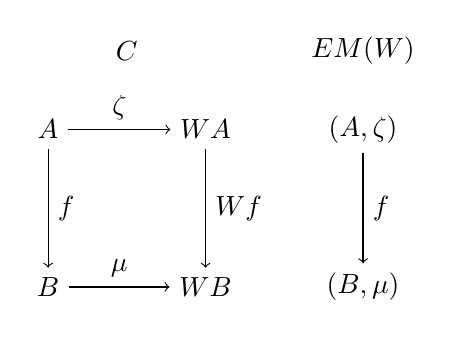
\begin{tikzpicture}[auto]
          \node (P) at (0, 0) {$A$};
          \node (Q) at (0, -2) {$B$};
          \node (TP) at (2, 0) {$WA$};
          \node (TQ) at (2, -2) {$WB$};
          \node (catpr) at (1, 1) {$\cat{C}$};

          \draw[->] (P) to node{$f$}(Q);
          \draw[->] (P) to node{$\zeta$}(TP);
          \draw[->] (TP) to node{$Wf$}(TQ);
          \draw[->] (Q) to node{$\mu$}(TQ);

          \node (P) at (4, 0) {$(A,\zeta)$};
          \node (Q) at (4, -2) {$(B,\mu)$};
          \draw[->] (P) to node{$f$}(Q);
          \node (cattam) at (4, 1) {$\cat{EM}(W)$};
        \end{tikzpicture}
      \end{center}
      \end{mydescription}
    \end{quote}
  \end{define}
  \begin{prop}
    $\cat{Tamb} = \cat{EM}(\Theta)$
  \end{prop}
  \begin{define}[自由忘却関手]
    圏$\cat{C}$上のコモナド$(W,\delta,\epsilon)$に対して忘却関手$\functor{U}{EM(W)}{C}$と自由関手$\functor{F}{C}{EM(W)}$を以下のように構成する。
    \begin{quote}
      \begin{mydescription}
        \item[対象関数] $U(A,\zeta)=A$
        \item[射関数] $U(f)=f$
        \begin{center}
          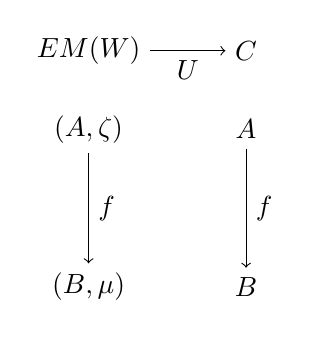
\begin{tikzpicture}[auto]
          \node (P) at (0, 0) {$A$};
          \node (Q) at (0, -2) {$B$};
          \node (catpr) at (0, 1) {$\cat{C}$};

          \draw[->] (P) to node{$f$}(Q);
          \node (P) at (-2, 0) {$(A,\zeta)$};
          \node (Q) at (-2, -2) {$(B,\mu)$};
          \draw[->] (P) to node{$f$}(Q);
          \node (cattam) at (-2, 1) {$\cat{EM}(W)$};
          \draw[<-] (catpr) to node{$U$}(cattam);

        \end{tikzpicture}
      \end{center}
      \end{mydescription}
    \end{quote}
    \begin{quote}
      \begin{mydescription}
        \item[対象関数] $F(A)=(WA,\delta_A)$
        \item[射関数] $F(f)=Wf$
        \begin{center}
          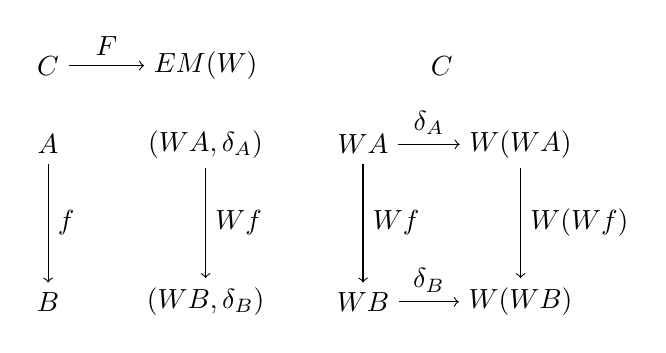
\begin{tikzpicture}[auto]
          \node (P) at (0, 0) {$A$};
          \node (Q) at (0, -2) {$B$};
          \node (catpr) at (0, 1) {$\cat{C}$};

          \draw[->] (P) to node{$f$}(Q);
          \node (P) at (2, 0) {$(WA,\delta_A)$};
          \node (Q) at (2, -2) {$(WB,\delta_B)$};
          \draw[->] (P) to node{$Wf$}(Q);
          \node (cattam) at (2, 1) {$\cat{EM}(W)$};
          \draw[->] (catpr) to node{$F$}(cattam);

          \node (wa) at (4, 0) {$WA$};
          \node (wb) at (4, -2) {$WB$};
          \node (wwa) at (6, 0) {$W(WA)$};
          \node (wwb) at (6, -2) {$W(WB)$};
          \node (catpr) at (5, 1) {$\cat{C}$};
          \draw[->] (wa) to node{$Wf$}(wb);
          \draw[->] (wwa) to node{$W(Wf)$}(wwb);
          \draw[->] (wa) to node{$\delta_A$}(wwa);
          \draw[->] (wb) to node{$\delta_B$}(wwb);

        \end{tikzpicture}
      \end{center}
      \end{mydescription}
    \end{quote}
  \end{define}
  \begin{prop}[余自由忘却随伴]
    関手$\functor{U}{EM(W)}{C},\ \functor{F}{C}{EM(W)}$は随伴関手である。
    \begin{quote}
      \begin{mydescription}
        \item[単位、余単位]
        単位、余単位となる自然変換$\nat{\eta}{Id}{FU},\ \nat{\epsilon}{UF}{Id}$を定義する。
        各々の成分を考えると$\mor{\eta_{(A,\zeta)}}{(A,\zeta)}{(WA,\delta_A)}$、$\mor{\epsilon_A}{WA}{A}$であり、
        \[\eta_{(A,\zeta)} = \zeta\]
        \[\epsilon_A = \epsilon_A\]とする。
        単位$\eta$はEM圏の対象の定義からEM圏における射の定義を満たし、自然性についても$\delta$の自然性とEM圏における射の定義により成り立つ。

        後者はそのままコモナド$(W,\delta,\epsilon)$の余単位子$\epsilon$を用いる。よってこれも自然になる。
        \item[三角恒等式]
        \[(F\circ\epsilon)\cdot(\eta\circ F) = ID_F\]
        \[(\epsilon\circ U)\cdot(U\circ\eta) = ID_U\]を満たせば良い。
        圏$\cat{C}$の任意の対象$A$に対して
        \begin{align*}
          ((F\circ\epsilon)\cdot(\eta\circ F))_A&=F(\epsilon_A)\circ(\eta_{FA})\\
          &=W\epsilon_A\circ\eta_{(A,\delta_A)}\\
          &=W\epsilon_A\circ\delta_A\\
          &=id_WA&\text{(コモナドの余単位則)}
        \end{align*}
        となる。よって$(F\circ\epsilon)\cdot(\eta\circ F) = ID_F$である。また圏$\cat{EM}(W)$の任意の対象$(A,\zeta)$に対して
        \begin{align*}
          ((\epsilon\circ U)\cdot(U\circ\eta))_{(A,\zeta)}
          &=\epsilon_{U(A,\zeta)}\circ U(\eta_{(A,\zeta)})\\
          &=\epsilon_A\circ U(\zeta)\\
          &=\epsilon_A\circ \zeta\\
          &=id_A&\text{(EM圏の対象の定義)}
        \end{align*}
        であるから$(\epsilon\circ U)\cdot(U\circ\eta) = ID_U$となる。
      \end{mydescription}
    \end{quote}
  \end{prop}
\end{document}